\begin{figure}[H]
    \begin{center}
        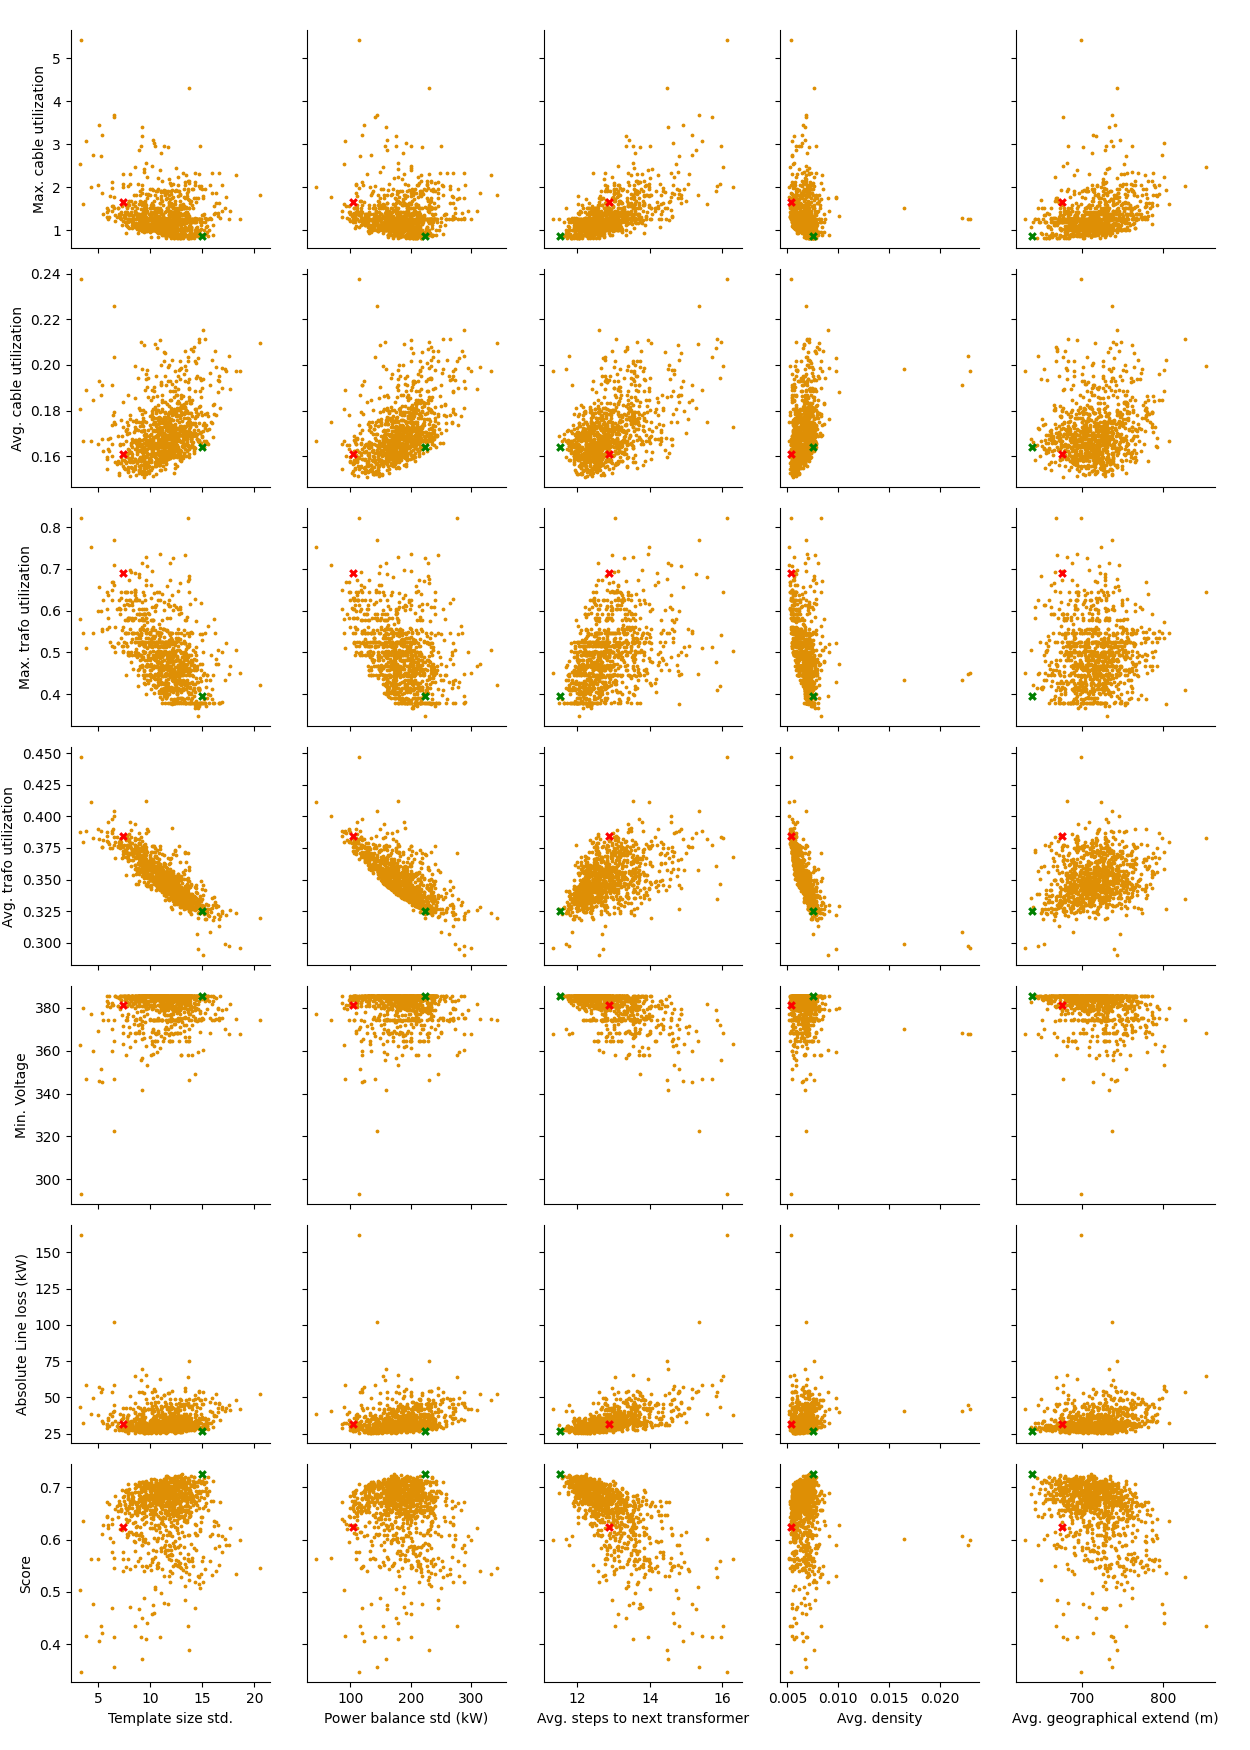
\includegraphics[width=\linewidth]{img/switchstate_exploring/swiss_suburb/correleation.png}
    \end{center}
    \caption{
        Correlation plots between topological/structural grid measures and 
        operational grid measures. Grid area as introduced In
        \autoref{fig:data_prep:swiss_suburb_topology_patched}.
        Data points in red are the SSS and in green the best random switch state.
        Refer to \autoref{sec:measures} for more
        information on the individual measures.
    }
    \label{fig:correlation}
\end{figure}

\autoref{fig:correlation} shows structural/topological grid
measures (\autoref{sec:topo_and_struct_measures}) vs. 
operational grid measures (\autoref{sec:operational_measures}). 
Some measures show almost linear relationships, like
the template size standard deviation (\autoref{sec:island_count}) vs.
the average transformer utilization. Other relations seem
to be fully random such as average geographical extend (\autoref{eq:measures:geo_extend})
vs. average cable utilization. Most relations lie in-between, there is
clearly some correlation, however it does not seem like it could
be captured through any simple formula.\\
\\
By far the most interesting relation that can be seen is 
average steps to the next transformer (\autoref{sec:shortest_path})
vs. score. The data seems to
suggest that the highest scores only exist at low average
step counts. It seems like a direct optimization for 
the average steps to the transformer could be performed in this grid
area instead for optimizing for score. As calculating the steps
is computationally cheaper than calculating the score this would
potentially allow for very fast optimization.\\
\\
Unfortunately these relations seem not to hold across grid areas
(compare \autoref{fig:appendix:suburb2:correleation} and \autoref{fig:appendix:suburb2:correleation}).
It seems like that the correlation between these measures is highly
dependent on the specific grid area examined. This means that
no universal optimizer optimizing for the presented
structural/topological measures can be developed.\\
\\
Further examination is certainly required, to determine if there
are any wider correlations holding across grid areas.

